\chapter{Methodology}
\label{chap:methodology}

In this chapter, we will cover the methodology used in this work. More details on the implementation in the application will be provided in Section \ref{sec:backend}.

\section{Pipeline Overview}
\label{sec:pipeline-overview}

The CryptoShow pipeline consists of several steps that work together to predict cryptic binding sites in protein structures and visualize them. The pipeline follows the steps outlined below, supported by Figure~\ref{fig:pipeline-overview}. The clustering, pocket smoothing and visualization steps are newly implemented in this thesis.

\begin{enumerate}
    \item \textbf{Structure Input} - The pipeline starts with a protein structure, which can be provided in PDB or mmCIF format. The structure can be obtained from the RCSB PDB database (see Section~\ref{sec:rcsb-pdb}), AlphaFold database (see Section~\ref{sec:alphafold-db}), or a custom structure file.
    \item \textbf{Sequence Extraction} - The sequence of the protein is extracted from the provided structure file. This step is important as the subsequent prediction model operates on sequence data.
    \item \textbf{Prediction} - The model used in CryptoBench (Section~\ref{sec:prediction}), referred to as \textbf{CB-Model}, is used to assign scores to individual residues on the protein sequence. The model generates residue-level predictions, which are then processed to identify potential binding site candidates.
    \item \textbf{Clustering} - The predicted residues are clustered (Section~\ref{sec:clustering}) to form potential cryptic binding sites (pockets). This is crucial for the visualization as coloring the clusters instead of just individual residues increases the interpretability of the results.
    \item \textbf{Pocket smoothing} - The pockets are then smoothed using a machine learning model (Section~\ref{sec:clustering}), which enhances the predictions by adding residues that are likely part of the cryptic binding site, even if their individual scores did not exceed the original high-scoring threshold.
    \item \textbf{Visualization} - The predicted cryptic binding sites are visualized in the frontend application (see Section \ref{sec:frontend}). The visualization includes the predicted binding sites and their associated scores. Also, the user can run an AHoJ query to retrieve apo-holo pairs of protein structures and visualize the trajectory animation of the conformational changes between the apo and holo structures.
\end{enumerate}

\begin{figure}[htbp]
    \centering
    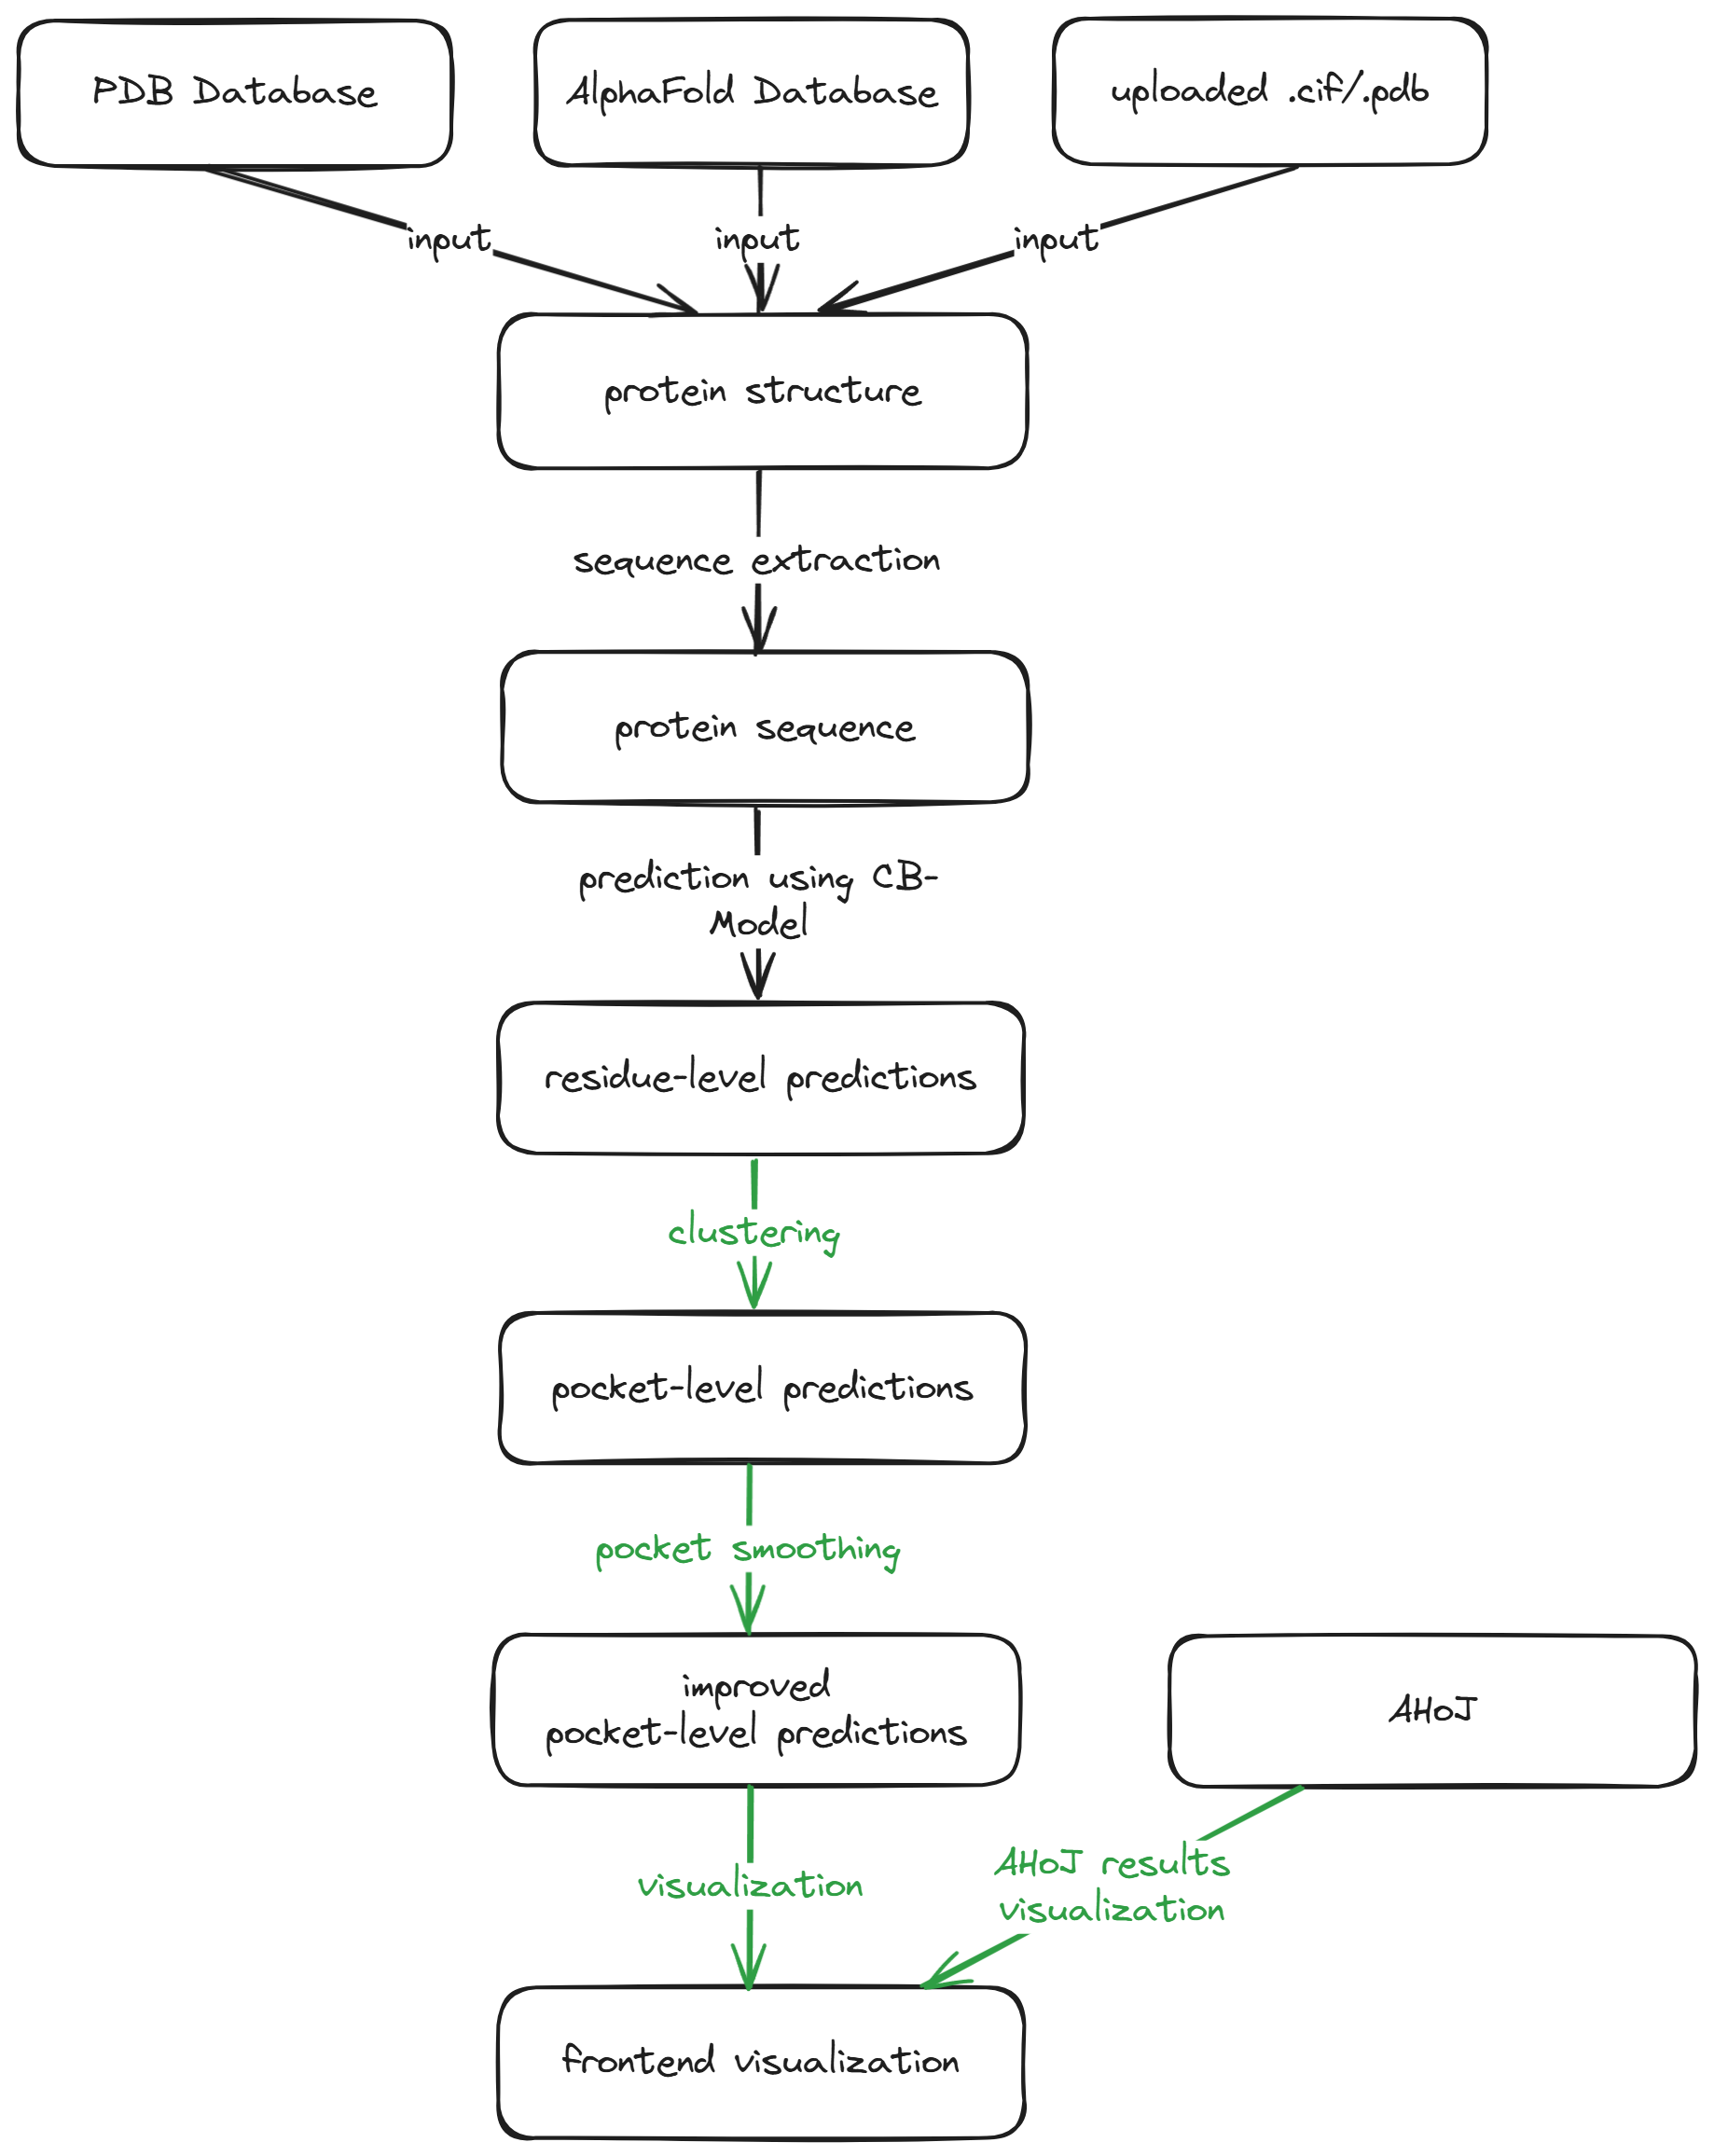
\includegraphics[width=\textwidth]{img/methodology-overview.png}
    \caption{Overview of the pipeline. The pipeline consists of several steps, starting with extraction of the sequence from a provided protein structure, followed by the prediction of cryptic binding sites using the CB-Model, followed by clustering and smoothing of the predictions, and finally querying AHoJ to retrieve relevant protein structures for trajectory animation. Steps marked with green arrows are newly implemented in this thesis.}
    \label{fig:pipeline-overview}
\end{figure}

\section{Protein Structure Input and Sequence Extraction}
\label{sec:structure-input}

The first step in the pipeline is to provide a protein structure in either PDB or mmCIF format. The structure can be obtained from the PDB database \cite{berman2000protein} or the AlphaFold database \cite{jumper2021highly}, or it can be a custom structure file. The structure is then parsed to extract the protein sequence for the CB-Model prediction.

\section{Prediction Using the CB-Model}
\label{sec:prediction}

The initial step in our methodology involves utilizing the CryptoBench \cite{vskrhak2025cryptobench} model to generate residue-level predictions for protein sequences. It is important to note that this model works solely with sequence information, without incorporating any structural (tertiary or quaternary) data. Specifically, we employ the tiny variant of CryptoBench\footnote{Available at \url{https://github.com/skrhakv/TinyCryptobench}} model, which is trained on a reduced version of the fine-tuned ESM-2 embeddings \cite{lin2022language} with 650 million parameters, as opposed to the full 3 billion. This choice is motivated by the observation that prediction accuracy remains comparable (according to the authors), while computational requirements are significantly reduced, enabling the pipeline to run efficiently on standard personal computers without the need for a GPU.

CryptoBench dataset was created by filtering the AHoJ-DB \cite{feidakis2024ahoj} dataset, which contains 57.8 million binding pockets (both apo and holo) \cite{apoholo-stats}. The filtering steps involved resolution filtering, removing redundant structures, geometric quality assurance, crypticity constraints, ligand filtering and sequence clustering. The final dataset consists of 1107 apo-holo pairs with 5493 cryptic binding sites. This dataset is used to train the model that has been benchmarked against PocketMiner \cite{meller2023predicting} and P2Rank \cite{krivak2018p2rank} and has shown better performance in terms of cryptic binding site prediction.


\section{Clustering and Smoothing}
\label{sec:clustering}

The next step in our methodology is to take the residue-level predictions generated by the CB-Model and cluster the high-scoring residues to form potential binding site candidates.

There are many algorithms available for clustering, namely DBSCAN \cite{schubert2017dbscan}, single-linkage clustering, hierarchical clustering \cite{jarman2020hierarchical}, and many more. In our case, we opted for the DBSCAN algorithm, which is a density-based clustering algorithm that groups together points that are closely packed together. This approach is particularly suitable for our use case, as it allows us to identify clusters of high-scoring residues without requiring a predefined number of clusters, and allows the specification of minimum residue distance and minimum number of residues in a cluster.

Our method relies on three parameters to control the clustering process:
\begin{itemize}
    \item \textbf{EPS ($\epsilon$)} - This parameter defines the maximum distance between two residues for them to be considered as part of the same cluster. In our case, we opted for a value of 5.0~\AA, which is a reasonable distance for residues when considering their spatial proximity in a protein structure as the average distance between the C$\alpha$ atoms in a protein structure is 3.8~\AA{} \cite{creighton1993proteins}.
    \item \textbf{Minimum cluster size} - This parameter defines the minimum number of residues required to form a cluster. We set this value to 3, as 2 residues are not sufficient to form a binding site candidate as the spatial complexity of a binding site is usually higher. This is also supported by the fact that less than 0.2\% of cryptic binding sites in the CryptoBench dataset have less than 3 residues.
    \item \textbf{Minimum (CB-Model) prediction score} - This parameter defines the minimum score a residue must have to be marked as a high-scoring residue. We opted for a value of 0.7 (inspired by the CryptoBench publication \cite{vskrhak2025cryptobench}), as this covers most of the dataset's binding residues, while also not marking the entire protein as a binding site candidate.
\end{itemize}

After the clustering is performed, we need to smoothen the clusters to enhance the predictions. This is caused by the fact that the clustering is performed only on the high-scoring residues, which can lead to missing residues in the binding site (as shown in Section~\ref{sec:pipeline-evaluation}, and in Figure~\ref{fig:smoothing-difference}). To address this, we collaborated with Vít Škrhák to develop an additional machine learning model. This model incorporates the protein sequence, the predicted clusters from the clustering step (along with sequence information), precomputed ESM-2 embeddings, and residue distance matrix derived from the structure file. Altogether, this \textbf{smoothing model} is then trained on a modified version of the CryptoBench dataset, using the annotated cryptic binding sites as the train and test set.

\begin{figure}
    \centering
    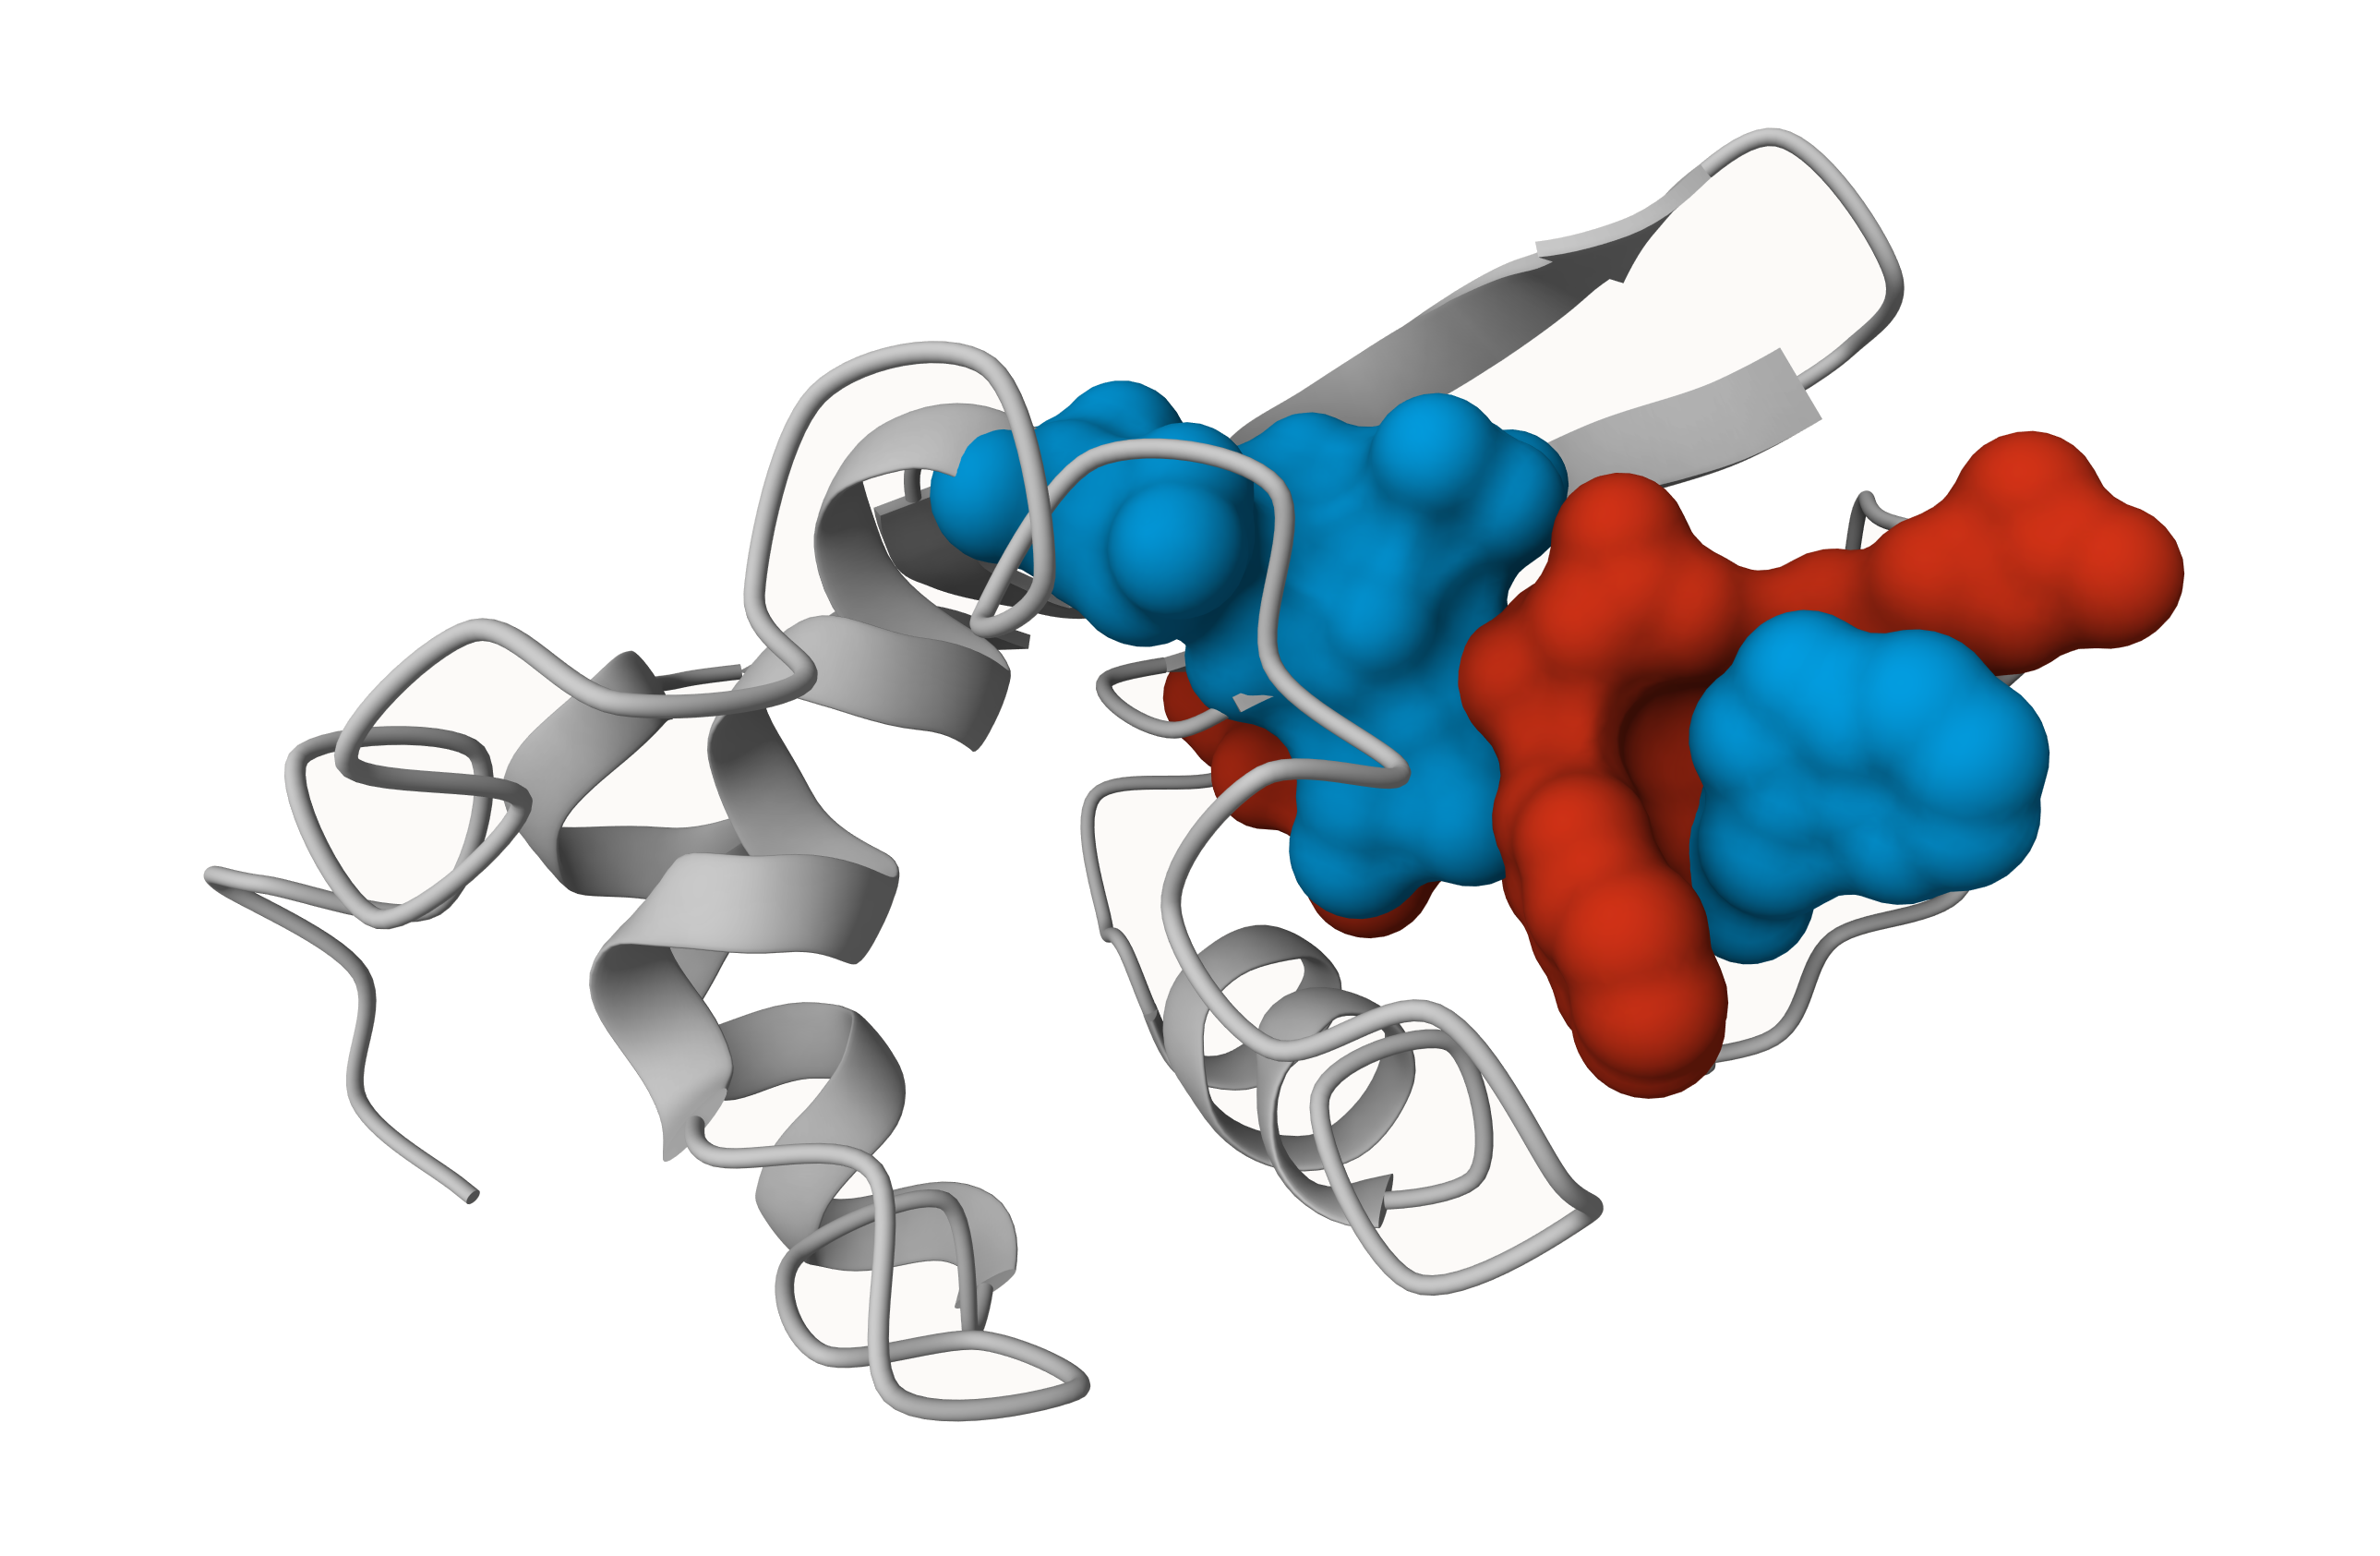
\includegraphics[width=0.8\textwidth]{img/smoothing-difference.png}
    \caption{Difference between the predicted cryptic binding site before and after the smoothing step in the 1LYZ protein structure (Real-space refinement of the structure of hen egg-white lysozyme). The residues colored in blue depict the residues predicted as binding by the CB-Model, while the residues colored in red are the residues added by the smoothing model. Visualized using Mol*.}
    \label{fig:smoothing-difference}
\end{figure}

The initial step involves preparing the dataset for training of the smoothing model. The dataset, consisting of 5493 cryptic binding sites, is split into training and testing sets using an 80:20 ratio. The sets follow the same structure as the CryptoBench dataset to prevent data leakage, i.e. the train set from CryptoBench is used as the train set for the smoothing model, and the test set from CryptoBench is used as the test set for the smoothing model. The test set is further filtered by the following criteria:

\begin{itemize}
    \item Pockets spanning multiple structure chains are omitted from the evaluation, as the process would be much more complicated and the prediction would require complex approaches.
    \item Many cryptic binding sites in the test set are similar to each other, which can lead to heavily inflated results. To address this, we have used the Szymkiewicz–Simpson coefficient (overlap), which is a measure of similarity between two sets $A, B$. The coefficient is defined in Equation~\ref{eq:szymkiewicz-simpson}.
    \begin{equation}
        \text{Szymkiewicz–Simpson}(A, B) = \frac{|A \cap B|}{\min(|A|, |B|)}
        \label{eq:szymkiewicz-simpson}
    \end{equation}
    After computing the overlap between each pair of cryptic binding sites in one structure, we keep only the CBSs with the overlaps under 0.5.
\end{itemize}

After the filtering, we have a test set of 193 apo conformations and 230 cryptic binding sites (out of the original 570 before the filtering).

Prior to training, it is essential to ensure that the precomputed embeddings from the previous step are available. Subsequently, the distance matrix for the residue coordinates must be calculated, which is accomplished using Equation~\ref{eq:distance-matrix}.

\begin{equation}
D_{ij} = \left\| \mathbf{c}_i - \mathbf{c}_j \right\|_2 = \sqrt{ \sum_{k=1}^3 (c_{ik} - c_{jk})^2 }
\label{eq:distance-matrix}
\end{equation}

where $D_{ij}$ denotes the Euclidean distance between residues $i$ and $j$, with $\mathbf{c}_i$ and $\mathbf{c}_j$ representing their respective 3D coordinates.

After the computation of the distance matrices, the next step involves generating both positive and negative training examples for the dataset. For the positive examples, residues are identified as candidates if their distance to any binding residue is less than a specified positive threshold (set to 15~\AA). For each such residue, a feature vector is constructed by combining its embedding with the mean embedding of its nearby binding neighbors. These feature vectors are then labeled as positive examples.

For negative examples, we identify residues that are located within a smaller threshold of 10~\AA{} from binding residues but are not themselves annotated as binding residues. These residues are labeled as negative examples. This strategy helps the model learn to differentiate between actual binding residues and nearby residues that do not participate in binding.

For training, we begin by calculating the class weights and loading the dataset. The neural network, which uses the same architecture described in Section \ref{sec:prediction}, is then trained. Cross-validation was not performed here primarily because the CryptoBench dataset is already partitioned into well-defined train and test sets, minimizing the risk of data leakage. Additionally, cross-validation would not provide significant additional benefit given the dataset's size and the existing split. Therefore, a straightforward train-test split was used, following the original CryptoBench partitioning. Evaluation of the model performance is described in Section~\ref{sec:pipeline-evaluation}.

The complete source code for the smoothing methodology can be found in the \inline|cryptoshow-benchmark/smoothing| directory. This includes scripts for model training, prepared training and testing datasets, inference, and an utility script for distance matrix computation.

\section{Pipeline Evaluation}
\label{sec:pipeline-evaluation}

After setting up the pipeline, we need to know if the clustering and smoothing steps perform well, i.e. if the final clusters correspond to actual binding sites. To address this, we have compared the clusters with the known binding sites from the CryptoBench test set, which contains 193 apo conformations and 230 cryptic binding sites (after filtering). The evaluation was performed in two steps: first, we benchmarked the clustering method without the smoothing model, and then we evaluated clustering including the smoothing model.

The evaluation follows the same procedure as the CryptoShow pipeline - first, the predictions are generated for each of the test set structures, then the clustering is performed. After creating the clusters, we compute the following metrics for each cluster, i.e. a predicted binding site, and compare them with the known binding sites:

\begin{itemize}
    \item \textbf{Distance between the predicted CBS center and the true CBS center (DCC)} - This metric is computed as the distance between the predicted CBS center and the center of the true CBS. Both centers are computed as the average of the 3D coordinates of the residues in the predicted CBS and the true CBS, respectively. The distance is computed in \AA. This is a standard metric used in evaluations of pocket prediction methods \cite{kandel2021puresnet}.
    \item \textbf{Percentage of true CBS residues covered by the predicted CBS} - This metric is computed as the percentage of residues in the true CBS that are also part of the predicted CBS.
    \item \textbf{Dice coefficient} - This metric is computed as the ratio of the number of residues in the intersection of the predicted CBS and the true CBS to the average number of residues in both sets $A, B$. It is defined in Equation~\ref{eq:dice-coefficient}.
    \begin{equation}
        \text{Dice}(A, B) = \frac{2 |A \cap B|}{|A| + |B|}
        \label{eq:dice-coefficient}
    \end{equation}
\end{itemize}

For each true CBS, after calculating the metrics against all predicted CBSs, the predicted CBS with the highest metric score is selected as the best match. After performing this procedure for all true CBSs and structures, we have plotted histograms to illustrate the performance of the clustering method. The results are visualized in Figure \ref{fig:clustering-benchmark}.

\begin{figure}[htbp]
    \centering
    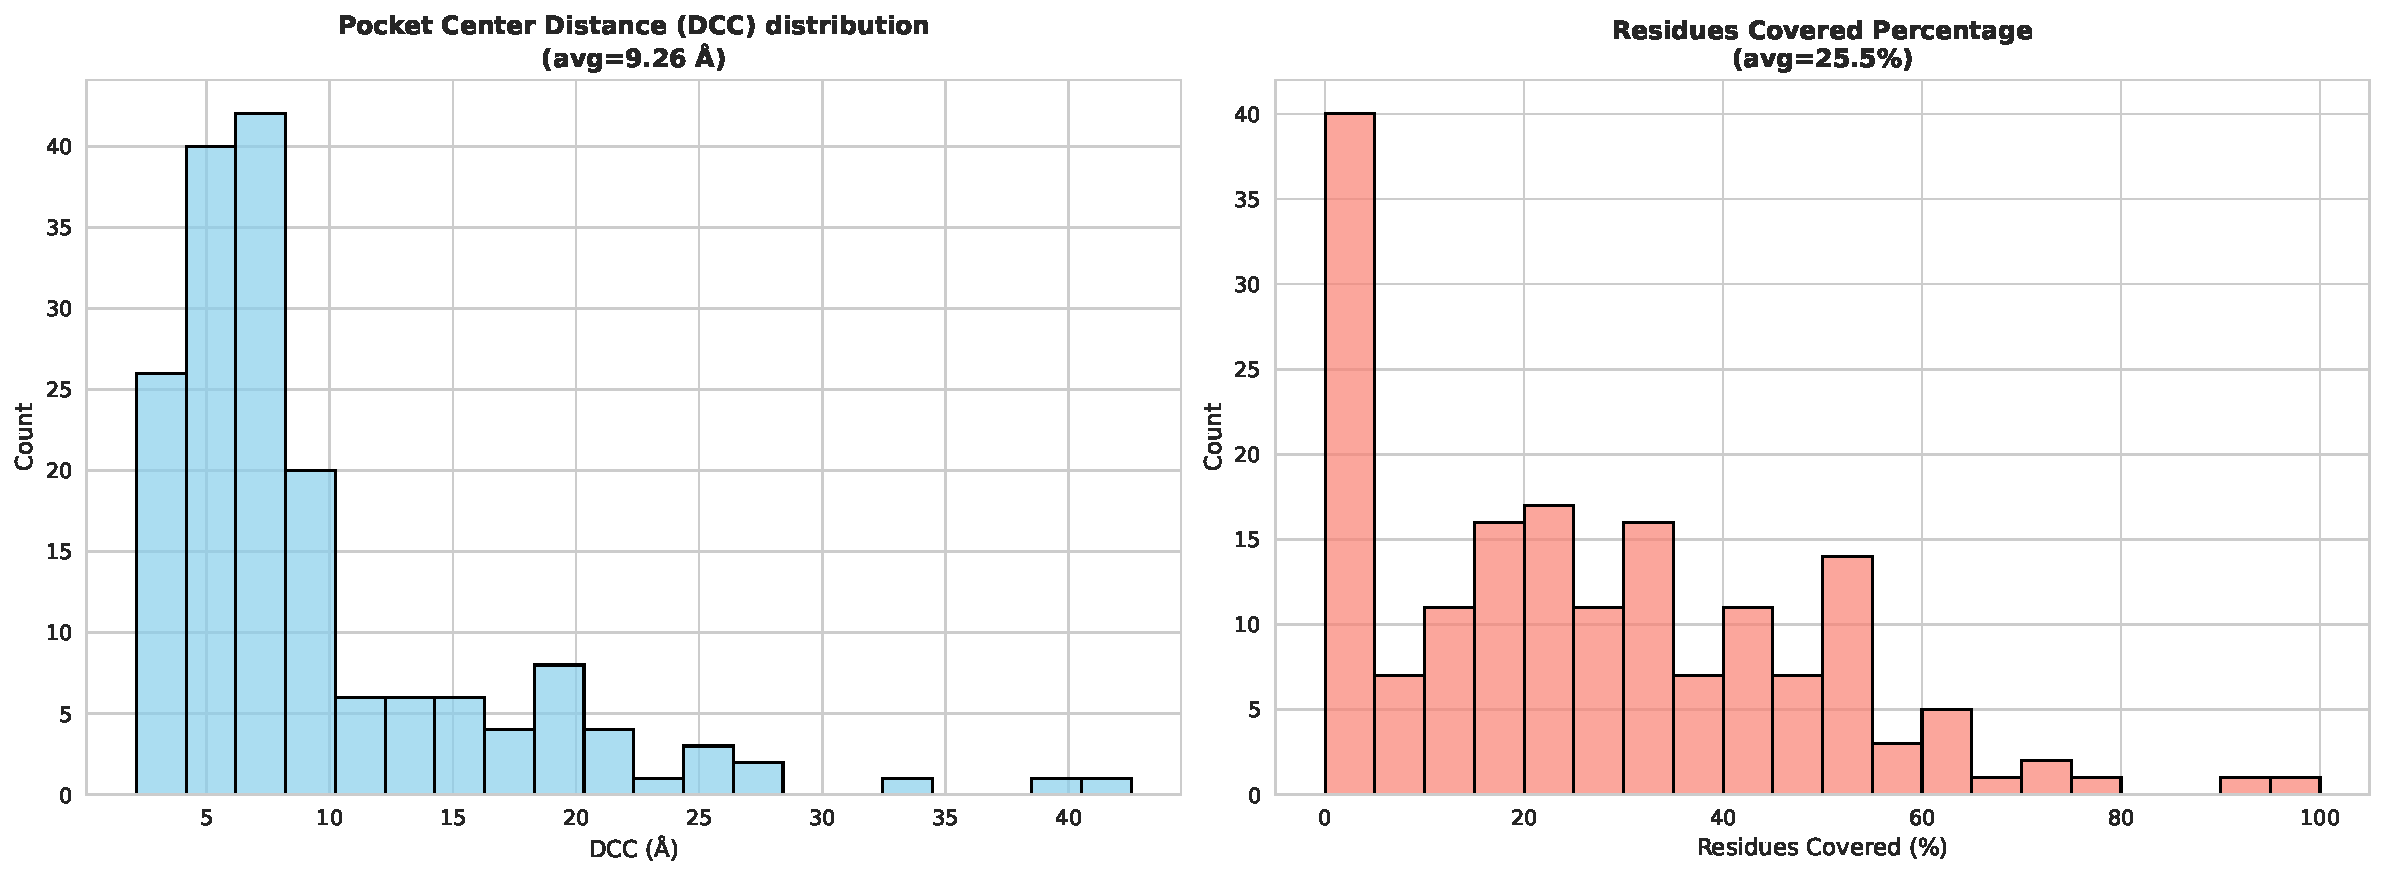
\includegraphics[width=\textwidth]{img/non-smoothened-1.pdf}
    \caption{Clustering benchmark results before pocket smoothing. The left plot shows the distance between the predicted CBS center and the true CBS center (DCC), and the right plot shows percentage of residues covered by the predicted CBSs.}
    \label{fig:clustering-benchmark}
\end{figure}

The results show that the clustering method without smoothing performs rather poorly, with the average DCC being around 10 \AA, and the percentage of true CBS residues covered by the predicted CBSs being around 25\%. This might not be a bad result as one missing residue in the binding site can lead to a significant increase in the distance, but the percentage of residues covered is rather low. This is caused by the fact that the clustering is performed only on the high-scoring residues. But, some of the true CBSs have residues with low scores (shown later in the section in Figure \ref{fig:clustering-benchmark-smoothened-dice}), which are still part of the binding site.

Now, we will evaluate the clustering method with the smoothing model included. The smoothing model is trained and tested on filtered version of the CryptoBench dataset, as described in Section~\ref{sec:clustering}. The smoothing model is evaluated on the test set, and the following metrics - F1 score, AUC, and accuracy (described in Equations \ref{eq:f1-score}, \ref{eq:auc}, and \ref{eq:accuracy}) - are computed for each threshold. Table~\ref{tab:smoothing-thresholds} and Figure~\ref{fig:smoothing-roc} illustrate the model's performance across various thresholds.

\begin{figure}[htpb]
    \centering
    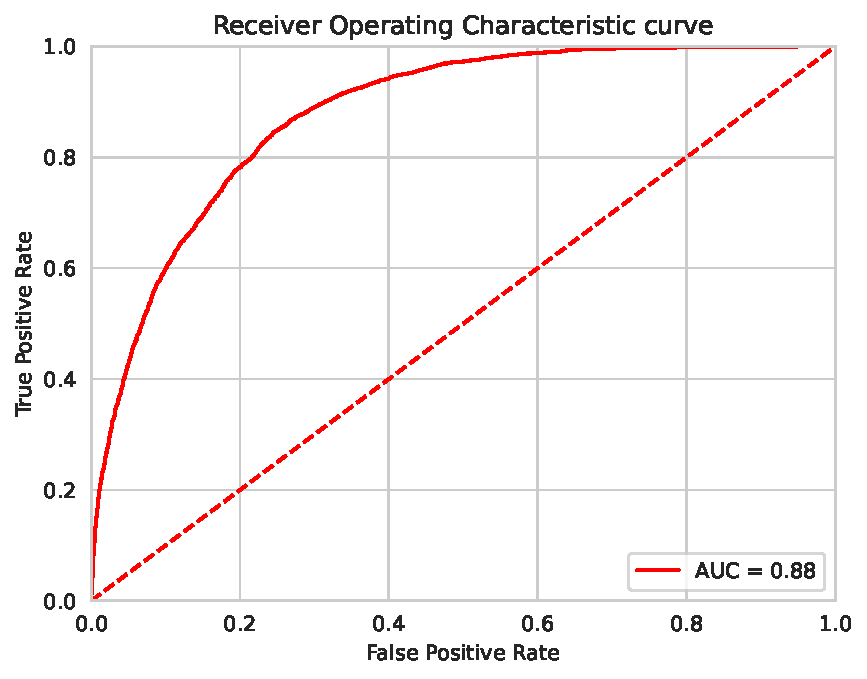
\includegraphics[width=0.65\textwidth]{img/smoothing-roc.pdf}
    \caption{Receiver Operating Characteristic (ROC) curve for the smoothing model.}
    \label{fig:smoothing-roc}
\end{figure}

\begin{equation}
\text{F1 score} = \frac{2 \cdot \text{precision} \cdot \text{recall}}{\text{precision} + \text{recall}}, \quad
\text{precision} = \frac{\text{TP}}{\text{TP} + \text{FP}}, \quad
\text{recall} = \frac{\text{TP}}{\text{TP} + \text{FN}}
\label{eq:f1-score}
\end{equation}

\begin{equation}
\text{AUC} = \int_0^1 \frac{\text{TP}(t)}{\text{TP}(t) + \text{FN}(t)} \, d\left( \frac{\text{FP}(t)}{\text{FP}(t) + \text{TN}(t)} \right)
\label{eq:auc}
\end{equation}

\begin{equation}
\text{Accuracy} = \frac{\text{TP} + \text{TN}}{\text{TP} + \text{TN} + \text{FP} + \text{FN}}
\label{eq:accuracy}
\end{equation}

where $\text{TP}$, $\text{TN}$, $\text{FP}$, and $\text{FN}$ denote true positives, true negatives, false positives, and false negatives.

\begin{table}[htbp]
    \centering
    \caption{Model performance metrics across different thresholds for the smoothing model.}
    \label{tab:smoothing-thresholds}
    \begin{tabular}{c|c|c}
        \hline
        \textbf{Threshold} & \textbf{F1 Score} & \textbf{Test Accuracy} \\
        \hline
        0.1 & 0.5875 & 55.09\% \\
        0.2 & 0.6787 & 64.16\% \\
        0.3 & 0.7369 & 70.51\% \\
        0.4 & 0.7777 & 75.24\% \\
        0.5 & 0.8051 & 78.64\% \\
        0.6 & 0.8266 & 81.55\% \\
        0.7 & 0.8417 & 83.93\% \\
        0.8 & 0.8413 & 85.04\% \\
        0.9 & 0.8163 & 84.57\% \\
        \hline
    \end{tabular}
\end{table}

During the smoothing step, the trained model is loaded and a threshold is set (with 0.7 chosen as the optimum based on the F1 score from the smoothing model evaluation, see Table~\ref{tab:smoothing-thresholds}). The relevant structure or sequence data is then prepared for inference. After running the model, the resulting smoothed pocket includes additional residues that are likely part of the cryptic binding site, even if their individual scores did not exceed the original high-scoring threshold.

The results demonstrate improved performance. As shown in Figures \ref{fig:clustering-benchmark-smoothened}, \ref{fig:clustering-benchmark-smoothened-dice}, the smoothing approach yields an average DCC of 5.12~\AA{} (a substantial improvement from 9.26~\AA{} without smoothing), an average residue coverage of 77.8\% (compared to the previous 25.5\%), and an average Dice coefficient of 0.51 (versus the earlier 0.32). These findings demonstrate that the smoothing methodology enhances prediction performance. While the predictions are not flawless, the majority of predicted pockets exhibit DCC within the 0 to 5~\AA{} range, representing a satisfactory outcome.

\begin{figure}[htbp]
    \centering
    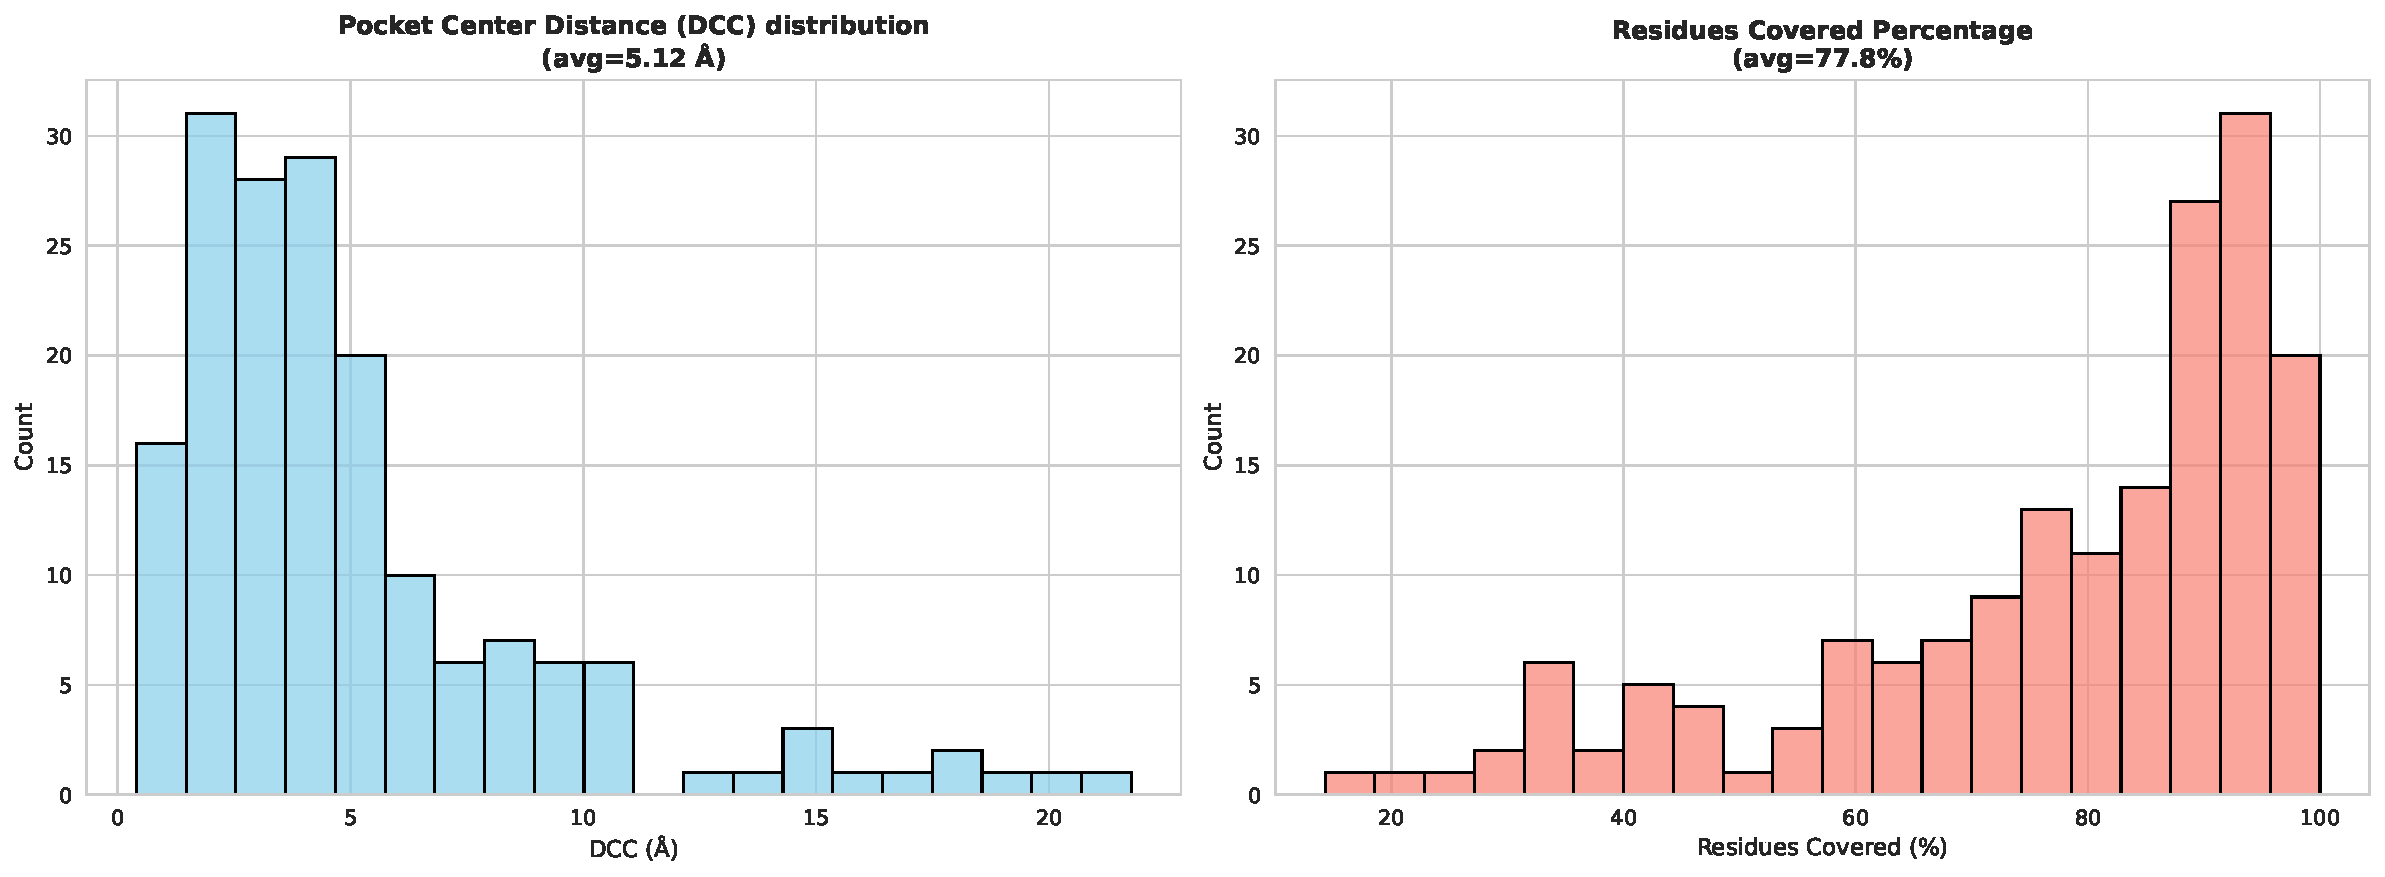
\includegraphics[width=\textwidth]{img/smoothened-1.pdf}
    \caption{Clustering benchmark results after pocket smoothing. The left plot shows the distance between the top-scoring predicted CBS center and the true CBS center (DCC), and the right plot shows percentage of residues covered by the predicted CBSs.}
    \label{fig:clustering-benchmark-smoothened}
\end{figure}

\begin{figure}[htbp]
    \centering
    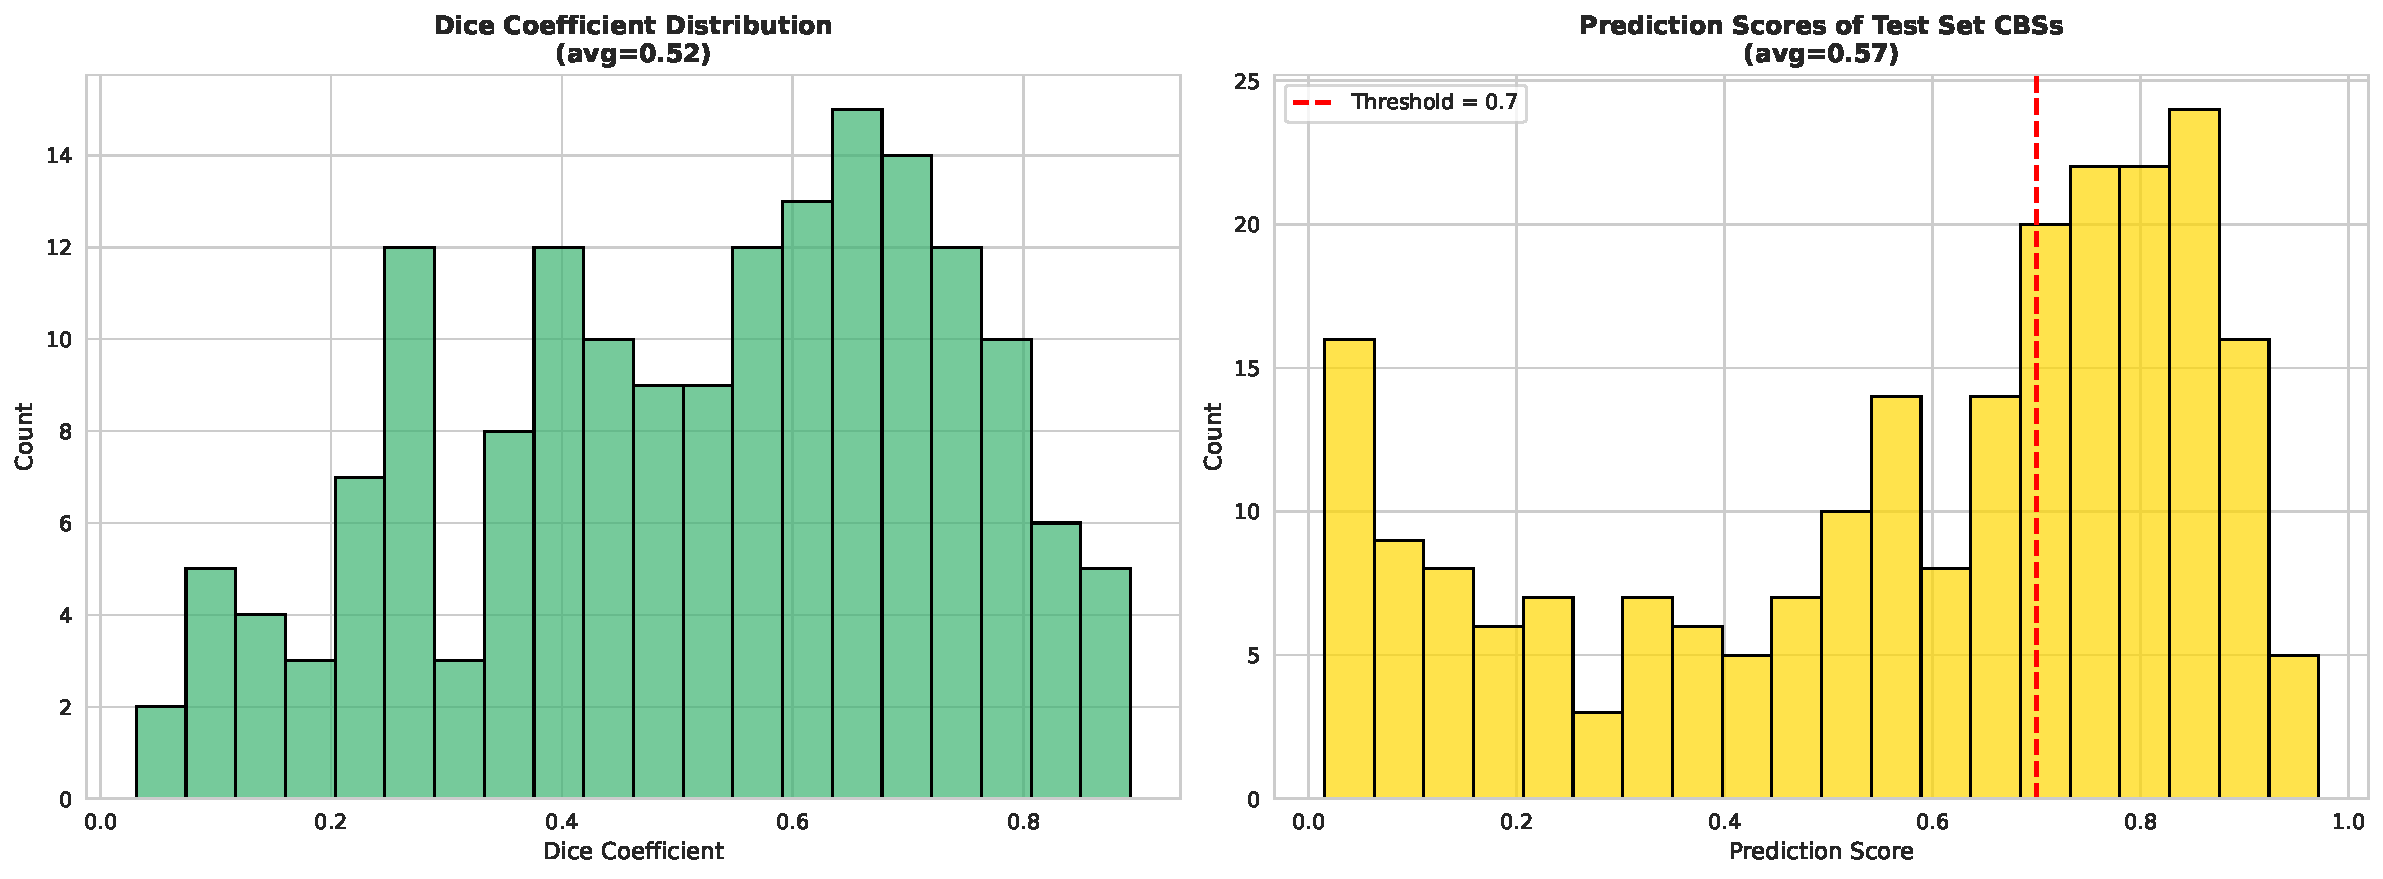
\includegraphics[width=\textwidth]{img/smoothened-2.pdf}
    \caption{Clustering benchmark results after pocket smoothing. The left plot shows the Dice coefficient between the top-scoring predicted CBS and true CBS. The right plot shows the distribution of prediction scores for all residues in the true CBSs.}
    \label{fig:clustering-benchmark-smoothened-dice}
\end{figure}

The evaluation notebooks including the full pipeline and other source codes are available in the \inline|cryptoshow-benchmark/benchmark_experiments| directory.
